% Created by tikzDevice version 0.6.2-92-0ad2792 on 2013-04-07 18:12:23
% !TEX encoding = UTF-8 Unicode
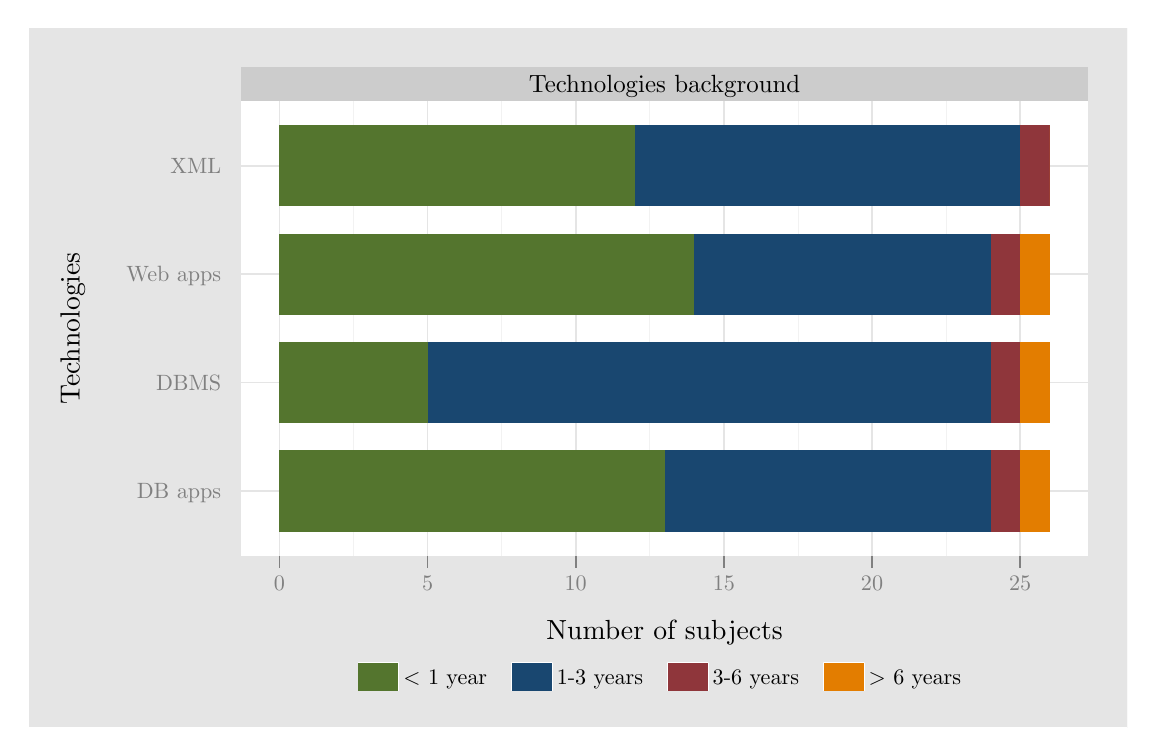
\begin{tikzpicture}[x=1pt,y=1pt]
\definecolor[named]{fillColor}{rgb}{1.00,1.00,1.00}
\path[use as bounding box,fill=fillColor,fill opacity=0.00] (0,0) rectangle (397.48,252.94);
\begin{scope}
\path[clip] (  0.00,  0.00) rectangle (397.48,252.94);
\definecolor[named]{drawColor}{rgb}{1.00,1.00,1.00}
\definecolor[named]{fillColor}{rgb}{0.90,0.90,0.90}

\path[draw=drawColor,line width= 0.6pt,line join=round,line cap=round,fill=fillColor] (  0.00,  0.00) rectangle (397.48,252.95);
\end{scope}
\begin{scope}
\path[clip] ( 77.04, 62.05) rectangle (383.26,226.50);
\definecolor[named]{fillColor}{rgb}{1.00,1.00,1.00}

\path[fill=fillColor] ( 77.04, 62.05) rectangle (383.26,226.50);
\definecolor[named]{drawColor}{rgb}{0.95,0.95,0.95}

\path[draw=drawColor,line width= 0.3pt,line join=round] (117.73, 62.05) --
	(117.73,226.50);

\path[draw=drawColor,line width= 0.3pt,line join=round] (171.26, 62.05) --
	(171.26,226.50);

\path[draw=drawColor,line width= 0.3pt,line join=round] (224.80, 62.05) --
	(224.80,226.50);

\path[draw=drawColor,line width= 0.3pt,line join=round] (278.33, 62.05) --
	(278.33,226.50);

\path[draw=drawColor,line width= 0.3pt,line join=round] (331.87, 62.05) --
	(331.87,226.50);
\definecolor[named]{drawColor}{rgb}{0.90,0.90,0.90}

\path[draw=drawColor,line width= 0.6pt,line join=round] ( 77.04, 85.54) --
	(383.26, 85.54);

\path[draw=drawColor,line width= 0.6pt,line join=round] ( 77.04,124.69) --
	(383.26,124.69);

\path[draw=drawColor,line width= 0.6pt,line join=round] ( 77.04,163.85) --
	(383.26,163.85);

\path[draw=drawColor,line width= 0.6pt,line join=round] ( 77.04,203.00) --
	(383.26,203.00);

\path[draw=drawColor,line width= 0.6pt,line join=round] ( 90.96, 62.05) --
	( 90.96,226.50);

\path[draw=drawColor,line width= 0.6pt,line join=round] (144.50, 62.05) --
	(144.50,226.50);

\path[draw=drawColor,line width= 0.6pt,line join=round] (198.03, 62.05) --
	(198.03,226.50);

\path[draw=drawColor,line width= 0.6pt,line join=round] (251.56, 62.05) --
	(251.56,226.50);

\path[draw=drawColor,line width= 0.6pt,line join=round] (305.10, 62.05) --
	(305.10,226.50);

\path[draw=drawColor,line width= 0.6pt,line join=round] (358.63, 62.05) --
	(358.63,226.50);
\definecolor[named]{fillColor}{rgb}{0.33,0.46,0.18}

\path[fill=fillColor] ( 90.96, 70.86) rectangle (230.15,100.22);
\definecolor[named]{fillColor}{rgb}{0.10,0.28,0.44}

\path[fill=fillColor] (230.15, 70.86) rectangle (347.93,100.22);
\definecolor[named]{fillColor}{rgb}{0.56,0.21,0.23}

\path[fill=fillColor] (347.93, 70.86) rectangle (358.63,100.22);
\definecolor[named]{fillColor}{rgb}{0.89,0.49,0.00}

\path[fill=fillColor] (358.63, 70.86) rectangle (369.34,100.22);
\definecolor[named]{fillColor}{rgb}{0.33,0.46,0.18}

\path[fill=fillColor] ( 90.96,110.01) rectangle (144.50,139.38);
\definecolor[named]{fillColor}{rgb}{0.10,0.28,0.44}

\path[fill=fillColor] (144.50,110.01) rectangle (347.93,139.38);
\definecolor[named]{fillColor}{rgb}{0.56,0.21,0.23}

\path[fill=fillColor] (347.93,110.01) rectangle (358.63,139.38);
\definecolor[named]{fillColor}{rgb}{0.89,0.49,0.00}

\path[fill=fillColor] (358.63,110.01) rectangle (369.34,139.38);
\definecolor[named]{fillColor}{rgb}{0.33,0.46,0.18}

\path[fill=fillColor] ( 90.96,149.17) rectangle (240.86,178.53);
\definecolor[named]{fillColor}{rgb}{0.10,0.28,0.44}

\path[fill=fillColor] (240.86,149.17) rectangle (347.93,178.53);
\definecolor[named]{fillColor}{rgb}{0.56,0.21,0.23}

\path[fill=fillColor] (347.93,149.17) rectangle (358.63,178.53);
\definecolor[named]{fillColor}{rgb}{0.89,0.49,0.00}

\path[fill=fillColor] (358.63,149.17) rectangle (369.34,178.53);
\definecolor[named]{fillColor}{rgb}{0.33,0.46,0.18}

\path[fill=fillColor] ( 90.96,188.32) rectangle (219.44,217.69);
\definecolor[named]{fillColor}{rgb}{0.10,0.28,0.44}

\path[fill=fillColor] (219.44,188.32) rectangle (358.63,217.69);
\definecolor[named]{fillColor}{rgb}{0.56,0.21,0.23}

\path[fill=fillColor] (358.63,188.32) rectangle (369.34,217.69);
\definecolor[named]{fillColor}{rgb}{0.89,0.49,0.00}

\path[fill=fillColor] (369.34,188.32) rectangle (369.34,217.69);
\end{scope}
\begin{scope}
\path[clip] (  0.00,  0.00) rectangle (397.48,252.94);
\definecolor[named]{fillColor}{rgb}{0.80,0.80,0.80}

\path[fill=fillColor] ( 77.04,226.50) rectangle (383.26,238.72);
\definecolor[named]{drawColor}{rgb}{0.00,0.00,0.00}

\node[text=drawColor,anchor=base,inner sep=0pt, outer sep=0pt, scale=  0.90] at (230.15,229.51) {Technologies background};
\end{scope}
\begin{scope}
\path[clip] (  0.00,  0.00) rectangle (397.48,252.94);
\definecolor[named]{drawColor}{rgb}{0.50,0.50,0.50}

\node[text=drawColor,anchor=base east,inner sep=0pt, outer sep=0pt, scale=  0.80] at ( 69.93, 82.79) {DB apps};

\node[text=drawColor,anchor=base east,inner sep=0pt, outer sep=0pt, scale=  0.80] at ( 69.93,121.94) {DBMS};

\node[text=drawColor,anchor=base east,inner sep=0pt, outer sep=0pt, scale=  0.80] at ( 69.93,161.09) {Web apps};

\node[text=drawColor,anchor=base east,inner sep=0pt, outer sep=0pt, scale=  0.80] at ( 69.93,200.25) {XML};
\end{scope}
\begin{scope}
\path[clip] (  0.00,  0.00) rectangle (397.48,252.94);
\definecolor[named]{drawColor}{rgb}{0.50,0.50,0.50}

\path[draw=drawColor,line width= 0.6pt,line join=round] ( 90.96, 57.78) --
	( 90.96, 62.05);

\path[draw=drawColor,line width= 0.6pt,line join=round] (144.50, 57.78) --
	(144.50, 62.05);

\path[draw=drawColor,line width= 0.6pt,line join=round] (198.03, 57.78) --
	(198.03, 62.05);

\path[draw=drawColor,line width= 0.6pt,line join=round] (251.56, 57.78) --
	(251.56, 62.05);

\path[draw=drawColor,line width= 0.6pt,line join=round] (305.10, 57.78) --
	(305.10, 62.05);

\path[draw=drawColor,line width= 0.6pt,line join=round] (358.63, 57.78) --
	(358.63, 62.05);
\end{scope}
\begin{scope}
\path[clip] (  0.00,  0.00) rectangle (397.48,252.94);
\definecolor[named]{drawColor}{rgb}{0.50,0.50,0.50}

\node[text=drawColor,anchor=base,inner sep=0pt, outer sep=0pt, scale=  0.80] at ( 90.96, 49.42) {0};

\node[text=drawColor,anchor=base,inner sep=0pt, outer sep=0pt, scale=  0.80] at (144.50, 49.42) {5};

\node[text=drawColor,anchor=base,inner sep=0pt, outer sep=0pt, scale=  0.80] at (198.03, 49.42) {10};

\node[text=drawColor,anchor=base,inner sep=0pt, outer sep=0pt, scale=  0.80] at (251.56, 49.42) {15};

\node[text=drawColor,anchor=base,inner sep=0pt, outer sep=0pt, scale=  0.80] at (305.10, 49.42) {20};

\node[text=drawColor,anchor=base,inner sep=0pt, outer sep=0pt, scale=  0.80] at (358.63, 49.42) {25};
\end{scope}
\begin{scope}
\path[clip] (  0.00,  0.00) rectangle (397.48,252.94);
\definecolor[named]{drawColor}{rgb}{0.00,0.00,0.00}

\node[text=drawColor,anchor=base,inner sep=0pt, outer sep=0pt, scale=  1.00] at (230.15, 31.70) {Number of subjects};
\end{scope}
\begin{scope}
\path[clip] (  0.00,  0.00) rectangle (397.48,252.94);
\definecolor[named]{drawColor}{rgb}{0.00,0.00,0.00}

\node[text=drawColor,rotate= 90.00,anchor=base,inner sep=0pt, outer sep=0pt, scale=  1.00] at ( 18.80,144.27) {Technologies};
\end{scope}
\begin{scope}
\path[clip] (  0.00,  0.00) rectangle (397.48,252.94);
\definecolor[named]{fillColor}{rgb}{0.90,0.90,0.90}

\path[fill=fillColor] (111.64,  9.15) rectangle (348.66, 27.65);
\end{scope}
\begin{scope}
\path[clip] (  0.00,  0.00) rectangle (397.48,252.94);
\definecolor[named]{drawColor}{rgb}{1.00,1.00,1.00}
\definecolor[named]{fillColor}{rgb}{1.00,1.00,1.00}

\path[draw=drawColor,line width= 0.6pt,line join=round,line cap=round,fill=fillColor] (119.52, 13.42) rectangle (133.97, 23.38);
\end{scope}
\begin{scope}
\path[clip] (  0.00,  0.00) rectangle (397.48,252.94);
\definecolor[named]{fillColor}{rgb}{0.33,0.46,0.18}

\path[fill=fillColor] (119.52, 13.42) rectangle (133.97, 23.38);

\path[] (119.52, 13.42) --
	(133.97, 23.38);
\end{scope}
\begin{scope}
\path[clip] (  0.00,  0.00) rectangle (397.48,252.94);
\definecolor[named]{drawColor}{rgb}{1.00,1.00,1.00}
\definecolor[named]{fillColor}{rgb}{1.00,1.00,1.00}

\path[draw=drawColor,line width= 0.6pt,line join=round,line cap=round,fill=fillColor] (174.94, 13.42) rectangle (189.39, 23.38);
\end{scope}
\begin{scope}
\path[clip] (  0.00,  0.00) rectangle (397.48,252.94);
\definecolor[named]{fillColor}{rgb}{0.10,0.28,0.44}

\path[fill=fillColor] (174.94, 13.42) rectangle (189.39, 23.38);

\path[] (174.94, 13.42) --
	(189.39, 23.38);
\end{scope}
\begin{scope}
\path[clip] (  0.00,  0.00) rectangle (397.48,252.94);
\definecolor[named]{drawColor}{rgb}{1.00,1.00,1.00}
\definecolor[named]{fillColor}{rgb}{1.00,1.00,1.00}

\path[draw=drawColor,line width= 0.6pt,line join=round,line cap=round,fill=fillColor] (231.28, 13.42) rectangle (245.74, 23.38);
\end{scope}
\begin{scope}
\path[clip] (  0.00,  0.00) rectangle (397.48,252.94);
\definecolor[named]{fillColor}{rgb}{0.56,0.21,0.23}

\path[fill=fillColor] (231.28, 13.42) rectangle (245.74, 23.38);

\path[] (231.28, 13.42) --
	(245.74, 23.38);
\end{scope}
\begin{scope}
\path[clip] (  0.00,  0.00) rectangle (397.48,252.94);
\definecolor[named]{drawColor}{rgb}{1.00,1.00,1.00}
\definecolor[named]{fillColor}{rgb}{1.00,1.00,1.00}

\path[draw=drawColor,line width= 0.6pt,line join=round,line cap=round,fill=fillColor] (287.63, 13.42) rectangle (302.09, 23.38);
\end{scope}
\begin{scope}
\path[clip] (  0.00,  0.00) rectangle (397.48,252.94);
\definecolor[named]{fillColor}{rgb}{0.89,0.49,0.00}

\path[fill=fillColor] (287.63, 13.42) rectangle (302.09, 23.38);

\path[] (287.63, 13.42) --
	(302.09, 23.38);
\end{scope}
\begin{scope}
\path[clip] (  0.00,  0.00) rectangle (397.48,252.94);
\definecolor[named]{drawColor}{rgb}{0.00,0.00,0.00}

\node[text=drawColor,anchor=base west,inner sep=0pt, outer sep=0pt, scale=  0.80] at (135.78, 15.64) {$<$ 1 year $\;\;$};
\end{scope}
\begin{scope}
\path[clip] (  0.00,  0.00) rectangle (397.48,252.94);
\definecolor[named]{drawColor}{rgb}{0.00,0.00,0.00}

\node[text=drawColor,anchor=base west,inner sep=0pt, outer sep=0pt, scale=  0.80] at (191.20, 15.64) {1-3 years $\;\;$};
\end{scope}
\begin{scope}
\path[clip] (  0.00,  0.00) rectangle (397.48,252.94);
\definecolor[named]{drawColor}{rgb}{0.00,0.00,0.00}

\node[text=drawColor,anchor=base west,inner sep=0pt, outer sep=0pt, scale=  0.80] at (247.54, 15.64) {3-6 years $\;\;$};
\end{scope}
\begin{scope}
\path[clip] (  0.00,  0.00) rectangle (397.48,252.94);
\definecolor[named]{drawColor}{rgb}{0.00,0.00,0.00}

\node[text=drawColor,anchor=base west,inner sep=0pt, outer sep=0pt, scale=  0.80] at (303.89, 15.64) {$>$ 6 years $\;\;$};
\end{scope}
\end{tikzpicture}
